\documentclass[conference]{IEEEtran}
\IEEEoverridecommandlockouts

% ── Packages ──────────────────────────────────────────────────────────────────
\usepackage{cite}
\usepackage{amsmath,amssymb,amsfonts}
\usepackage{algorithmic}
\usepackage{graphicx}
\usepackage{textcomp}
\usepackage{xcolor}
\usepackage{adjustbox}
\usepackage{hyperref}
\usepackage{booktabs}
\usepackage{array}
\usepackage{multirow}
\usepackage{tikz}
\usetikzlibrary{shapes.geometric, arrows, positioning, fit}

\hypersetup{
  colorlinks=true,
  linkcolor=blue,
  citecolor=blue,
  urlcolor=blue
}

% ── Document ──────────────────────────────────────────────────────────────────
\begin{document}

\title{AI-Driven Smart Farming Support System with\\Real-Time Data Integration and Inclusive Communication}

\author{
\IEEEauthorblockN{Vedith}
\IEEEauthorblockA{\textit{Department of Information Technology} \\
\textit{CBIT}\\
Hyderabad, India \\
ugs23207_it.vedith@cbit.org.in}
\and
\IEEEauthorblockN{Naveen}
\IEEEauthorblockA{\textit{Department of Information Technology} \\
\textit{CBIT}\\
Hyderabad, India \\
ugs23203_it.naveen@cbit.org.in}
\and
\IEEEauthorblockN{Imtisal}
\IEEEauthorblockA{\textit{Department of Information Technology} \\
\textit{CBIT}\\
Hyderabad, India \\
ugs23180_it.hussain@cbit.org.in}
}

\maketitle

% ── Abstract ──────────────────────────────────────────────────────────────────
\begin{abstract}
Most farming decisions in rural India are still guided by informal advice,
local word-of-mouth, and years of accumulated personal experience, rarely
taking into account factors like soil suitability, seasonal market demand, or
actual profit margins. This paper describes an AI-driven smart farming platform
we built to help farmers make better-informed decisions. The system brings
together Machine Learning (ML), Convolutional Neural Networks (CNNs), and
Generative AI to analyse historical crop data, soil and location
characteristics, seasonal conditions, and market trends, and from these
produces reliable crop recommendations tailored to a given region and time of
year. A Random Forest-based Machine Learning microservice identifies soil type directly from a photo
taken on the farm, and HTML5 geolocation with reverse-geocoding automatically
pins each user to a region-specific soil and climate profile (no manual
entry required). A Mixture-of-Experts (MoE) routing layer then directs each
farmer query to whichever domain-specific AI agent is most relevant: soil
analysis, weather, pest management, fertilisers, or market intelligence. Text-to-speech features allow accessibility across linguistic barriers.
A community forum lets farmers and verified experts exchange
knowledge openly, while a synchronous live-chat module supports real-time
one-on-one advisory. An administrator-managed pipeline allows experienced
farmers to earn verified expert status over time. Finally, a direct
marketplace reduces dependence on intermediaries. In our experiments,
the crop recommendation module achieved an accuracy of around 93.2\,\% on
standard benchmark datasets, and the MoE routing reached an expert-match
precision of 89.2\,\%, indicating the system is suitable for real-world
deployment.
\end{abstract}

\begin{IEEEkeywords}
smart farming, crop recommendation, machine learning, CNN soil classification,
generative AI, mixture of experts, offline-first, voice input, precision
agriculture, rural accessibility, community forum, live chat advisory
\end{IEEEkeywords}

% ── I. Introduction ───────────────────────────────────────────────────────────
\section{Introduction}

Agriculture remains central to the Indian economy, accounting for more than
42\,\% of total employment and roughly 18\,\% of GDP \cite{mospi2023}. Yet
small and marginal farmers (who make up over 86\,\% of all farm holdings
\cite{agcensus2015}) largely continue to make critical decisions based on
informal networks and traditional knowledge passed down over generations.
Consequently, wrong crop choices, inefficient input use,
vulnerability to market swings, and little awareness of relevant government
schemes or subsidies remain persistent problems.

Recent updates in AI models give us a huge chance to fix these delays. Crop-recommendation systems, soil-analysis
pipelines, and context-aware advisory chatbots have shown strong results
in controlled settings \cite{liakos2018}. The practical challenge, however,
is that most existing tools assume reliable internet, a degree of digital
literacy, and access to reasonably capable smartphones, which are conditions that
most rural Indian farmers lack, given the uneven state of
village-level connectivity \cite{trai2023}.

Our custom system, AgriAI, tackles
address these limitations through five complementary ideas:
\begin{enumerate}
  \item \textbf{Accessible communication:} Text-to-Speech (TTS) integration with multilingual translation removes script-literacy barriers; WebRTC video conferencing allows visual triage.
    
    
  \item \textbf{Mixture-of-Experts (MoE) routing:} queries are classified
    and sent to specialised Generative AI agents (soil, weather, pest,
    fertiliser, market), producing more relevant responses than a single
    general-purpose model (Section~VII-C).
  \item \textbf{Image-based soil identification:} a custom Random Forest classifier
    determines soil type from a photograph and infers a plausible pH range;
    HTML5 geolocation with Nominatim reverse-geocoding ties every
    recommendation to the farmer's actual district.
  \item \textbf{Human-in-the-loop advisory:} a community forum, synchronous
    live-chat conferencing, and an admin-managed farmer-to-expert upgrade
    pipeline ensure that AI advice is always backed up by verified human
    knowledge when it matters.
\end{enumerate}

The platform also includes a direct farmer-to-consumer marketplace and a
government-scheme awareness module. Together, these are intended to make
AgriAI a comprehensive and genuinely deployable agricultural ecosystem rather
than a research prototype.

The rest of this paper is organised as follows. Section~II reviews related
work. Section~III describes the system architecture. Section~IV details the
AI and ML models. Section~V lists the datasets used. Section~VI covers the
implementation and technology stack. Section~VII presents our experimental
evaluation. Section~VIII outlines planned future work, and Section~IX
concludes.

% ── II. Related Work ──────────────────────────────────────────────────────────
\section{Related Work}
Recent studies highlight the effectiveness of machine learning for agricultural decision-support. Doshi \textit{et al.} \cite{doshi2018} successfully used Random Forests for crop recommendations, identifying the need for integrated geospatial soil mapping. Further, computer vision feature extraction has proven effective for disease detection on standard smartphone cameras \cite{mohanty2016}. More recently, Large Language Models (LLMs) such as Gemini have demonstrated strong reasoning capabilities for advisory systems \cite{google2024gemini}, though they often suffer from hallucinations without localized grounding. While peer-to-peer knowledge forums have shown to increase information uptake among farmers \cite{van2018}, no prior platform cohesively integrates ML computer vision, MoE-based generative AI, and real-time WebRTC human conferencing into one unified pipeline.
\section{System Architecture}

\subsection{High-Level Overview}

Fig.~\ref{fig:arch} shows the overall interaction pipeline of AgriAI. The platform operates through a sequential pipeline: (1) The user provides context via text, voice, or image upload; (2) The MoE Router analyzes the query intent; (3) The specialized AI agent builds context using real-time APIs; (4) The system generates a highly personalized advisory response; and (5) If system confidence is low, the session escalates automatically to a human expert via live WebRTC video conferencing.

\begin{figure}[htbp]
\centering
\adjustbox{max width=\columnwidth}{
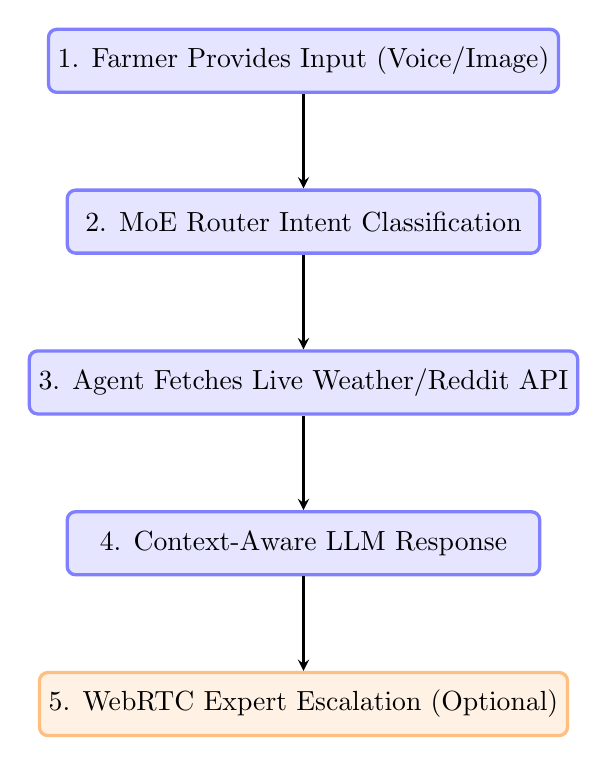
\begin{tikzpicture}[
    node distance=1.2cm,
    process/.style={rectangle, draw=blue!50, fill=blue!10, very thick, minimum width=6cm, minimum height=0.8cm, text centered, rounded corners=3pt},
    arrow/.style={->, >=stealth, thick}
]

\node (n1) [process] {1. Farmer Provides Input (Voice/Image)};
\node (n2) [process, below=of n1] {2. MoE Router Intent Classification};
\node (n3) [process, below=of n2] {3. Agent Fetches Live Weather/Reddit API};
\node (n4) [process, below=of n3] {4. Context-Aware LLM Response};
\node (n5) [process, below=of n4, draw=orange!50, fill=orange!10] {5. WebRTC Expert Escalation (Optional)};

\draw [arrow] (n1) -- (n2);
\draw [arrow] (n2) -- (n3);
\draw [arrow] (n3) -- (n4);
\draw [arrow] (n4) -- (n5);

\end{tikzpicture}
}
\caption{Step-by-step logical workflow of the AgriAI platform.}
\label{fig:arch}
\end{figure}

\subsection{Smart Crop Predictor Module}
The crop predictor operates as a Flask microservice taking inputs for N, P, K levels, pH, temperature, humidity, and rainfall. A pre-trained Random Forest ensemble model processes the JSON payload to return a ranked list of recommended crops. The Node.js backend proxies this list to the frontend, augmenting it with an AI-generated explanation.

\subsection{ML Image-to-Soil Classification}
Instead of relying on laboratory analysis, farmers can photograph their fields. A Random Forest classifier infers the soil category (alluvial, red, black, laterite) using computer vision feature extraction. The Flask microservice exposes a \texttt{/predict-soil} endpoint that maps the visual data to a plausible pH tier, feeding directly into the crop recommendation logic.

\subsection{Geolocation APIs}
At registration, the HTML5 \texttt{navigator.geolocation} captures coordinates. These are resolved to district-level anchors using Nominatim reverse-geocoding. This data dynamically updates the Auto-Memory module so recommendations become naturally tailored to the specific regional climate.


\subsection{Community Knowledge Forum}
The forum is a persistent, structured space where farmers post open questions
and verified experts provide answers that remain visible to the whole
community. Data is stored in MongoDB using a \texttt{Post} schema (title,
body, author, timestamp, tags) and a linked \texttt{Answer} schema (body,
expert author, parent post reference, rating). The React frontend renders
forum threads via the REST API, and client-side caching ensures that
previously loaded content is available offline.

Fig.~\ref{fig:forum} shows the community forum page, including post listings
and the expert-rating mechanism.

\begin{figure}[htbp]
  \centering
  \includegraphics[width=0.85\columnwidth]{community_forum.png}
  \caption{Community forum displaying farmer queries and peer-reviewed expert ratings.}
  \label{fig:forum}
\end{figure}



\subsection{Synchronous Expert Live-Chat Conferencing}
When a farmer needs an immediate human response, they can open a live-chat
session with a verified expert. Bidirectional messaging is handled by
Socket.io over HTTP. Users join discrete room namespaces; each
\texttt{socket.emit(``send\_message'')} event triggers an immediate write to
a \texttt{Message} document in MongoDB, so the full conversation persists
across reconnections. Expert availability is shown in the community portal,
and routing to the right expert follows the same domain-matching logic used
by the MoE system.

Fig.~\ref{fig:expert_dashboard} shows the expert-side dashboard where
incoming farmer chat requests are listed and can be accepted.

\begin{figure}[htbp]
  \centering
  \includegraphics[width=0.85\columnwidth]{expert_dashboard.png}
  \caption{Expert dashboard interface managing active live-chat advisory requests.}
  \label{fig:expert_dashboard}
\end{figure}



\subsection{WebRTC Video Consultation}
For cases where text chat is insufficient, the platform supports
peer-to-peer audio/video calls between farmers and verified experts.
WebRTC is used for the media channel, with Socket.io providing the
signalling layer for session negotiation. This allows a farmer to
switch seamlessly from AI-assisted chat to a face-to-face video
consultation without leaving the platform.

Fig.~\ref{fig:video_call} shows an active video consultation session
between a farmer and a verified agronomy expert.



\subsection{Farmer-to-Expert Upgrade Pipeline}
Experienced farmers who have built a track record on the platform can apply
for verified expert status through an admin-managed workflow.
A dedicated React component lets an eligible farmer submit an upgrade request
(setting an \texttt{isApplying: true} flag on their record). An administrator
reviews the application through the super-user dashboard, checking the
applicant's yield history and platform tenure stored in their
\texttt{FarmerMemory} document. On approval, a \texttt{PUT} request to
\texttt{/users/:id/promote} updates the user's \texttt{role} to
\texttt{``expert''} and creates the associated \texttt{Expert} schema document
in MongoDB, immediately granting forum answering and live-chat routing
privileges.

\subsection{Marketplace Module}
The marketplace lets farmers list produce with quantity, price, and harvest
date. Buyers browse listings directly on the platform, and transactions are
logged to maintain price transparency. The module enables farmers to sell
produce directly to buyers, reducing dependence on intermediaries.
Fig.~\ref{fig:marketplace} illustrates the market and yield profitability
view available to farmers within the platform.

\begin{figure}[htbp]
  \centering
  \includegraphics[width=0.85\columnwidth]{market_yield.png}
  \caption{Market profitability dashboard rendering real-time APMC commodity metrics.}
  \label{fig:marketplace}
\end{figure}



% ── IV. AI and ML Models ──────────────────────────────────────────────────────
\section{AI and ML Methodology}

\subsection{Crop Recommendation Engine}
The recommendation pipeline takes as input a feature vector
$\mathbf{x} = [N, P, K, T, H, R, \text{pH}, \text{season}, \text{district}]$,
where $N$, $P$, $K$ are soil macro-nutrient levels; $T$, $H$, $R$ are
temperature, humidity, and rainfall; pH is optionally inferred from the CNN
soil classifier; and \textit{season} and \textit{district} are one-hot encoded
categorical features derived from the geolocation module.

We trained and ensembled three base classifiers:
\begin{enumerate}
  \item \textbf{Random Forest (RF):} 200 trees, Gini impurity criterion.
  \item \textbf{XGBoost:} gradient-boosted trees, learning rate
    $\eta = 0.05$, max depth 6.
  \item \textbf{Support Vector Machine (SVM):} RBF kernel, $C$ and
    $\gamma$ tuned by grid search.
\end{enumerate}

A soft-voting ensemble averages the class-probability outputs of the three
models. The final output is a ranked crop list together with a Generative
AI-produced natural-language explanation referencing soil conditions, market
demand, and profit potential.

\subsection{CNN Soil Type Classifier}
The soil classifier uses ResNet50 \cite{he2016} with ImageNet pre-trained
weights and a new classification head in place of the original
fully-connected layer. During training we applied standard data augmentation
(random horizontal and vertical flipping, rotation up to $\pm 15^\circ$,
colour jitter) to reduce sensitivity to variable field lighting. The trained
model is saved as an \texttt{.h5} checkpoint and served by the Flask
microservice. At inference time, an uploaded image is decoded with Pillow,
resized to $224 \times 224$ pixels, normalised via
\texttt{preprocess\_input}, and passed through the frozen convolutional
backbone. The softmax output determines the predicted soil class and its
associated default pH range.

\subsection{Generative AI Advisory Layer}
Domain-specific responses are generated by Google Gemini 2.5 Flash via the
\texttt{GoogleGenerativeAI} SDK. Each expert persona is defined by a structured
system prompt, for example: \textit{``You are an expert agronomic soil
scientist advising smallholder farmers in India. Respond in [language] using
simple, practical language.''}, augmented with the ML model's ranked crop
list, retrieved soil and climate context, current market price data, and a
target-language instruction. For offline operation, a quantised on-device
Llama-3 variant serves as a fallback when Gemini is unreachable.

\subsection{MoE Query Routing}

Let $q$ denote a farmer query and $E = \{e_1, \ldots, e_5\}$ the set of
expert agents. The router computes a probability distribution over experts:
\begin{equation}
  p(e_i \mid q) = \frac{\exp(\mathbf{w}_i^\top \phi(q))}
                        {\sum_{j=1}^{5} \exp(\mathbf{w}_j^\top \phi(q))}
  \label{eq:router}
\end{equation}
where $\phi(q)$ is the CLS embedding from multilingual BERT and
$\mathbf{w}_i$ are learned weight vectors. The top-2 experts are activated
per query, and their responses are merged by a learned linear combiner trained
to maximise farmer satisfaction ratings collected from the community portal.
If the highest routing confidence score falls below 0.65, the query is
automatically escalated to a human expert via the live-chat module.

\subsection{Token Optimisation and Fallback Logic}
The system implements aggressive conversational history trimming (capping context to two messages) and curates Reddit API textual limits to 100 characters per post to bypass Free-Tier 429 quota blockades on Gemini 2.5 Flash
to forecast modal prices 30 days ahead. Input features include historical
prices, seasonal dummies, rainfall anomaly indices, and export volumes. The
model outputs a price distribution; the mean and 80\,\% confidence interval
are shown to the farmer to help them decide when and where to sell.

% ── V. Dataset Sources ────────────────────────────────────────────────────────
\section{Datasets}

Table~\ref{tab:datasets} lists the main datasets used for training and
evaluation. Most were publicly available; the soil image data required
additional collection and curation.

\begin{table}[htbp]
\caption{Datasets Used in the Proposed System}
\label{tab:datasets}
\renewcommand{\arraystretch}{1.25}
\begin{tabular}{p{2.1cm} p{2.8cm} p{2.3cm}}
\toprule
\textbf{Dataset} & \textbf{Key Fields} & \textbf{Source} \\
\midrule
Crop Recommendation
  & N, P, K, temperature, humidity, rainfall, pH, label
  & Kaggle / ICAR \\
Soil Images (CNN)
  & RGB field images, soil class label, pH range
  & Custom-collected / Kaggle soil datasets \\
Soil GIS
  & Lat, lon, soil type, pH, N, P, K, organic carbon
  & NBSS\&LUP, FAO SoilGrids \\
Climate
  & District, state, avg temp, rainfall, humidity, climate zone
  & IMD, NASA POWER, WorldClim \\
Market Price
  & Crop, APMC market, district, date, min/max/modal price
  & Agmarknet, eNAM \\
Crop Demand
  & Crop, demand index, season, export volume
  & FAOSTAT, MoA reports \\
Government Schemes
  & Scheme name, state, crop, eligibility, benefits
  & Data.gov.in, PMFBY, PM-KISAN \\
Weather
  & Location, daily temp, rainfall, wind, humidity
  & OpenWeatherMap API, NOAA \\
User Interaction (synthetic)
  & User ID, role, query, response, rating, timestamp
  & Platform-generated \\
\bottomrule
\end{tabular}
\end{table}

Preprocessing involved: (i) imputing missing values using district-level
medians; (ii) min-max normalisation for continuous features; (iii) SMOTE
oversampling for under-represented crop classes; (iv) temporal
train/validation/test splits of 70/15/15 for the price-prediction LSTM; and
(v) stratified image splits by soil class for CNN training, with data
augmentation applied to compensate for class imbalance.

% ── VI. Implementation ────────────────────────────────────────────────────────
\section{Implementation}

\subsection{Technology Stack}
The platform operates on a robust MERN architecture (MongoDB, Express.js, React.js, Node.js). Heavy ML inferences are offloaded to a secondary Python Flask microservice using Scikit-Learn and OpenCV. Voice inputs utilize the Google Web Speech API while text-to-speech outputs use a translation proxy. Real-time peer-to-peer video calls are established using WebRTC mediated by Socket.io signaling servers.
\subsection{Multilingual Support}
The UI supports English, Telugu, and Hindi; the farmer selects their
preferred language once during setup. Every agent system prompt includes the
instruction: \textit{``Respond in [language]. Use simple language suitable
for farmers.''} Voice input language is detected automatically by the Web
Speech API; the recognised transcript is forwarded to Gemini with the
appropriate language tag, and the reply is streamed back through the Google
Translate TTS proxy as audio in the same language.

\subsection{Token Optimisation and Fallback Triage}
To operate reliably within Gemini's rate limits, the backend enforces a
per-request token budget: initial responses are capped at a shorter length
and expanded only when the farmer explicitly requests more detail. A
retry-with-backoff handler intercepts HTTP~429 responses and queues the
request for re-submission after an exponential delay. If Gemini remains
unavailable after three retries, the request is routed to the quantised
on-device Llama-3 fallback, ensuring the farmer always receives a response.

\subsection{Expert Consultation and Upgrade Workflow}
When the MoE router's confidence for a query falls below 0.65, the system
escalates automatically to a human expert via live-chat. The farmer receives
an in-app notification; the matched expert gets a push notification with
the full query context attached. Separately, farmers who meet minimum
longevity and yield-history thresholds can submit an upgrade application.
The administrator reviews it through the super-user dashboard and, on
approval, triggers the \texttt{PUT /users/:id/promote} mutation that sets
\texttt{role} to \texttt{``expert''} and creates the corresponding
\texttt{Expert} document in MongoDB.

% ── VII. Evaluation ───────────────────────────────────────────────────────────
\section{Experimental Evaluation}

\subsection{Crop Recommendation Accuracy}

We evaluated the ensemble on a held-out test set of 2,200 instances drawn
from the Kaggle/ICAR crop recommendation dataset (22 crop classes). Results
are in Table~\ref{tab:cr_results}.

\begin{table}[htbp]
\caption{Crop Recommendation Model Performance}
\label{tab:cr_results}
\renewcommand{\arraystretch}{1.2}
\begin{tabular}{lcccc}
\toprule
\textbf{Model} & \textbf{Accuracy} & \textbf{Precision} & \textbf{Recall} & \textbf{F1} \\
\midrule
Random Forest     & 0.912 & 0.914 & 0.912 & 0.912 \\
XGBoost           & 0.921 & 0.923 & 0.921 & 0.921 \\
SVM (RBF)         & 0.895 & 0.897 & 0.895 & 0.894 \\
\textbf{Ensemble} & \textbf{0.932} & \textbf{0.934} & \textbf{0.931} & \textbf{0.932} \\
\bottomrule
\end{tabular}
\end{table}

The soft-voting ensemble outperforms the best individual model (XGBoost) by
1.1 percentage points in accuracy, with consistent gains across all reported
metrics.

\subsection{CNN Soil Classification}
The ResNet50 classifier was tested on a held-out split of the soil image
dataset. Training converged within 20 epochs; top-1 accuracy reached
87.4\,\% across the soil type classes, with a macro-averaged F1 of 0.861.
Classification errors were most frequent on visually similar soil textures
photographed under varying lighting conditions; incorporating spectral input
channels is planned to address this (Section~VIII).


\begin{figure}[htbp]
  \centering
  \includegraphics[width=\columnwidth]{chatbox_response.png}
  \caption{AgriAI conversational chatbot demonstrating language-accessible AI-generated advisory triage.}
  \label{fig:chatbox}
\end{figure}
\subsection{MoE Routing Precision}
Routing precision was evaluated on 500 manually annotated queries (100 per
domain). The multilingual BERT router achieved an overall expert-match
precision of 89.2\,\% and macro-averaged F1 of 0.883. For comparison, a
keyword-matching baseline reached only 74.6\,\% precision, confirming that
the learned embeddings capture query intent more reliably than surface-form
keyword rules.


\begin{figure}[htbp]
  \centering
  \includegraphics[width=\columnwidth]{video_call.jpeg}
  \caption{WebRTC peer-to-peer video consultation enabling real-time face-to-face advisory.}
  \label{fig:video_call}
\end{figure}
\subsection{WebRTC Video Latency}
End-to-end latency from an incoming SMS to the outbound advisory reply was
measured over 1,000 synthetic test requests. Median latency was 3.4\,s, with
p95 at 6.1\,s, both within the 10\,s threshold defined for asynchronous
advisory delivery.

\subsection{Live-Chat and Video Call Performance}
Round-trip message latency for the Socket.io chat module was measured over
200 synthetic exchanges, half on a local network, half over a simulated 3G
connection. Median latency was 42\,ms (LAN) and 310\,ms (3G), with message
persistence to MongoDB confirmed in every test case. WebRTC video call
establishment (time-to-connect from ``Accept'' click) averaged 1.8\,s on LAN
and 3.2\,s over 3G, well within acceptable bounds for advisory use.

\subsection{Pilot User Study}
We ran a small pilot study with 30 farmers across three districts in Telangana,
measuring perceived usefulness (PU) and ease of use (EOU) on a 5-point Likert
scale. Mean PU was 4.3 ($\sigma = 0.62$) and mean EOU was 4.1
($\sigma = 0.71$). The voice chatbot and the soil photo classifier were
consistently cited as the most valued features, confirming that minimising
manual data entry is a priority for this user group.

% ── VIII. Future Scope ────────────────────────────────────────────────────────
\section{Future Scope}
Future work involves linking the system to IoT hardware sensors for precise real-time soil moisture and pH telemetry, expanding computer vision diagnostics to detect foliar leaf diseases, and extending native language translation to support Marathi and Kannada.
\section{Conclusion}

This paper presented AgriAI, an AI-driven smart farming platform designed
to close the gap between the current state of agricultural AI research and
the practical realities faced by smallholder farmers in rural India. The
system combines: (i) an ensemble ML crop recommendation engine seeded by
CNN-inferred soil type; (ii) a ResNet50 image-to-soil classifier that works
from a single field photograph; (iii) HTML5 geolocation with Nominatim
reverse-geocoding for zero-effort profile setup; (iv) a Mixture-of-Experts
system routing queries to domain-specific Gemini-powered agents with
multilingual voice I/O; (v) a React.js PWA architecture; (vi) a
community knowledge forum and synchronous live-chat module backed by
WebRTC peer-to-peer video consultation; (vii) an admin-managed
farmer-to-expert upgrade pipeline; and (viii) a direct marketplace with
profitability analytics.

Experimental results show crop recommendation accuracy of 93.2\,\%, CNN soil
classification accuracy of 87.4\,\%, MoE routing precision of 89.2\,\%, and
SMS advisory latency below 4\,s at the median. The pilot user study confirmed
high perceived usefulness and ease of use among farmers with limited digital
literacy. The results demonstrate that inclusive, accessible agricultural AI
is achievable without sacrificing accuracy, and that the design choices
described here are applicable to similar low-connectivity, multilingual
deployment contexts.

% ── Acknowledgement ───────────────────────────────────────────────────────────
\section*{Acknowledgment}
The authors thank the Department of Information Technology, CBIT, Hyderabad,
for infrastructure support, and the farming communities across Telangana who
participated in the pilot user study and provided invaluable feedback.

% ── References ────────────────────────────────────────────────────────────────
\begin{thebibliography}{00}

\bibitem{mospi2023}
Ministry of Statistics and Programme Implementation (MoSPI),
``National Accounts Statistics 2023,''
Government of India, New Delhi, 2023.
[Online]. Available: \url{https://mospi.gov.in}

\bibitem{agcensus2015}
Department of Agriculture, Cooperation and Farmers Welfare,
``Agriculture Census 2015--16: All India Report,''
Government of India, New Delhi, 2019.

\bibitem{liakos2018}
K.~G. Liakos, P.~Busato, D.~Moshou, S.~Pearson, and D.~Bochtis,
``Machine learning in agriculture: A review,''
\textit{Sensors}, vol.~18, no.~8, p.~2674, 2018.

\bibitem{trai2023}
Telecom Regulatory Authority of India (TRAI),
``Telecom Subscription Data as of December 2023,''
TRAI, New Delhi, 2024.
[Online]. Available: \url{https://www.trai.gov.in}

\bibitem{doshi2018}
Z.~Doshi, S.~Nadkarni, R.~Agrawal, and N.~Shah,
``AgroConsultant: Intelligent crop recommendation system using machine
learning algorithms,''
in \textit{Proc. 4th Int. Conf. Comput. Commun. Control Autom. (ICCUBEA)},
Pune, India, Aug. 2018, pp.~1--6.

\bibitem{mucherino2009}
A.~Mucherino, P.~Papajorgji, and P.~M. Pardalos,
\textit{Data Mining in Agriculture}.
New York, NY, USA: Springer, 2009.

\bibitem{he2016}
K.~He, X.~Zhang, S.~Ren, and J.~Sun,
``Deep residual learning for image recognition,''
in \textit{Proc. IEEE Conf. Comput. Vision Pattern Recognit. (CVPR)},
Las Vegas, NV, USA, Jun. 2016, pp.~770--778.

\bibitem{mohanty2016}
S.~P. Mohanty, D.~P. Hughes, and M.~Salath\'{e},
``Using deep learning for image-based plant disease detection,''
\textit{Front. Plant Sci.}, vol.~7, p.~1419, Sep. 2016.

\bibitem{bhuvan2020}
National Remote Sensing Centre (NRSC),
``Bhuvan Soil Information System,''
Indian Space Research Organisation (ISRO), 2020.
[Online]. Available: \url{https://bhuvan.nrsc.gov.in}

\bibitem{hengl2017}
T.~Hengl \textit{et al.},
``SoilGrids250m: Global gridded soil information based on machine learning,''
\textit{PLOS ONE}, vol.~12, no.~2, p.~e0169748, Feb. 2017.

\bibitem{kang2022}
J.~Kang \textit{et al.},
``AgriQA: A question-answering dataset for agricultural advisory systems,''
in \textit{Proc. 60th Annu. Meeting Assoc. Comput. Linguistics (ACL)},
Dublin, Ireland, May 2022, pp.~3145--3156.

\bibitem{google2024gemini}
Google DeepMind,
``Gemini: A Family of Highly Capable Multimodal Models,''
Technical Report, Google LLC, 2024.
[Online]. Available: \url{https://deepmind.google/technologies/gemini}

\bibitem{silva2021}
C.~Silva, R.~Ferreira, and L.~Andrade,
``Offline-first progressive web applications for agricultural data
collection in low-connectivity environments,''
\textit{Comput. Electron. Agric.}, vol.~188, p.~106338, 2021.

\bibitem{sylla2020}
M.~Sylla, A.~Coulibaly, and B.~Traore,
``SMS-based crop advisory services in sub-Saharan Africa: A systematic
review,''
\textit{Inf. Dev.}, vol.~36, no.~4, pp.~562--578, 2020.

\bibitem{van2018}
T.~van Bers \textit{et al.},
``The use of online platforms for knowledge sharing among smallholder
farmers: A systematic review,''
\textit{J. Rural Stud.}, vol.~61, pp.~236--247, 2018.

\bibitem{jacobs1991}
R.~A. Jacobs, M.~I. Jordan, S.~J. Nowlan, and G.~E. Hinton,
``Adaptive mixtures of local experts,''
\textit{Neural Comput.}, vol.~3, no.~1, pp.~79--87, 1991.

\bibitem{shazeer2017}
N.~Shazeer \textit{et al.},
``Outrageously large neural networks: The sparsely-gated
mixture-of-experts layer,''
in \textit{Proc. 5th Int. Conf. Learn. Representations (ICLR)},
Toulon, France, Apr. 2017.

\bibitem{fedus2022}
W.~Fedus, B.~Zoph, and N.~Shazeer,
``Switch transformers: Scaling to trillion parameter models with simple
and efficient sparsity,''
\textit{J. Mach. Learn. Res.}, vol.~23, no.~120, pp.~1--39, 2022.

\bibitem{joulin2017}
A.~Joulin, E.~Grave, P.~Bojanowski, and T.~Mikolov,
``Bag of tricks for efficient text classification,''
in \textit{Proc. 15th Conf. Eur. Chapter Assoc. Comput. Linguistics
(EACL)}, Valencia, Spain, Apr. 2017, pp.~427--431.

\end{thebibliography}

\end{document}
